%%%%%%%%%%%%%%%%%%%%%%%%%%%%%%%%%%%%%%%%%%%%%%%%%%%%%%%%%%%%%%%%%%%%%%%%%%%%%%%
\chapter{Advocating for Multiple Defense Strategies against Adversarial Examples}
\label{chapter:advocating_multiple_defense_strategies_against_adversarial_examples}
%%%%%%%%%%%%%%%%%%%%%%%%%%%%%%%%%%%%%%%%%%%%%%%%%%%%%%%%%%%%%%%%%%%%%%%%%%%%%%%
\localtoc

% \begin{abstract}
%   It has been empirically observed that defense mechanisms designed to protect neural networks against $\linf$ adversarial examples offer poor performance against $\ltwo$ adversarial examples and vice versa. In this paper we conduct a geometrical analysis that validates this observation. Then, we provide a number of empirical insights to illustrate the effect of this phenomenon in practice. 
%   Then, we review some of the existing defense mechanism that attempts to defend against multiple attacks by mixing defense strategies. Thanks to our numerical experiments, we discuss the relevance of this method and state open questions for the adversarial examples community.
% \end{abstract}

\emph{This Appendix concerns a collaboration ..}

\todo{write short context}


%%%%%%%%%%%%%%%%%%%%%%%%%%%%%%%%%%%%%%%%%%%%%%%%%%%%%%%%%%%%%%%%%%%%%%%%%%%%%%%
\section{Introduction}
\label{section:ap4-introduction}
%%%%%%%%%%%%%%%%%%%%%%%%%%%%%%%%%%%%%%%%%%%%%%%%%%%%%%%%%%%%%%%%%%%%%%%%%%%%%%%

Deep neural networks achieve state-of-the-art performances in a variety of domains such as natural language processing~\cite{radford2018Language}, image recognition~\cite{he2016deep} and speech recognition~\cite{hinton2012deep}.
However, it has been shown that such neural networks are vulnerable to \emph{adversarial examples}, \ie, imperceptible variations of the natural examples, crafted to deliberately mislead the models~\cite{globerson2006nightmare,biggio2013evasion,szegedy2013intriguing}.
Since their discovery, a variety of algorithms have been developed to generate adversarial examples (\aka attacks), for example FGSM \cite{goodfellow2014explaining}, PGD \cite{madry2018towards} and C\&W \cite{carlini2017towards}, to mention the most popular ones.

Because it is difficult to characterize the space of visually imperceptible variations of a natural image, existing adversarial attacks use surrogates that can differ from one attack to another.
For example, \citet{goodfellow2014explaining} use the $\linf$ norm to measure the distance between the original image and the adversarial image whereas \citet{carlini2017towards} use the $\ltwo$ norm.
When the input dimension is low, the choice of the norm is of little importance because the $\linf$ and $\ltwo$ balls overlap by a large margin, and the adversarial examples lie in the same space.
An important insight in this paper is to observe that the overlap between the two balls  diminishes exponentially quickly as the dimensionality of the input space increases.
For typical image datasets with large dimensionality, the two balls are mostly disjoint.
As a consequence, the $\linf$ and the $\ltwo$ adversarial examples lie in different areas of the space, and it explains why $\linf$ defense mechanisms perform poorly against $\ltwo$ attacks and vice versa. 

Building on this insight, we advocate for designing models that incorporate defense mechanisms against both $\linf$ and $\ltwo$ attacks and review several ways of mixing existing defense mechanisms.
In particular, we evaluate the performance of  {\em Mixed Adversarial Training} (MAT)~\cite{goodfellow2014explaining} which consists of  augmenting training batches using \emph{both} $\linf$ and $\ltwo$ adversarial examples, and {\em Randomized Adversarial Training} (RAT)~\cite{salman2019provably}, a solution to benefit from the advantages of both $\linf$ adversarial training, and $\ltwo$ randomized defense. 


%%%%%%%%%%%%%%%%%%%%%%%%%%%%%%%%%%%%%%%%%%%%%%%%%%%%%%%%%%%%%%%%%%%%%%%%%%%%%%%
\section{No Free Lunch for Adversarial Defenses}
\label{section:ap4-no_free_lunch}
%%%%%%%%%%%%%%%%%%%%%%%%%%%%%%%%%%%%%%%%%%%%%%%%%%%%%%%%%%%%%%%%%%%%%%%%%%%%%%%

In this Section, we show both theoretically and empirically that defenses mechanisms intending to defend against $\linf$ attacks cannot provide suitable defense against $\ltwo$ attacks.
Our reasoning is perfectly general; hence we can similarly demonstrate the reciprocal statement, but we focus on this side for simplicity.


\begin{figure}
   \centering
   \begin{subfigure}[b]{0.32\textwidth}
       \centering
       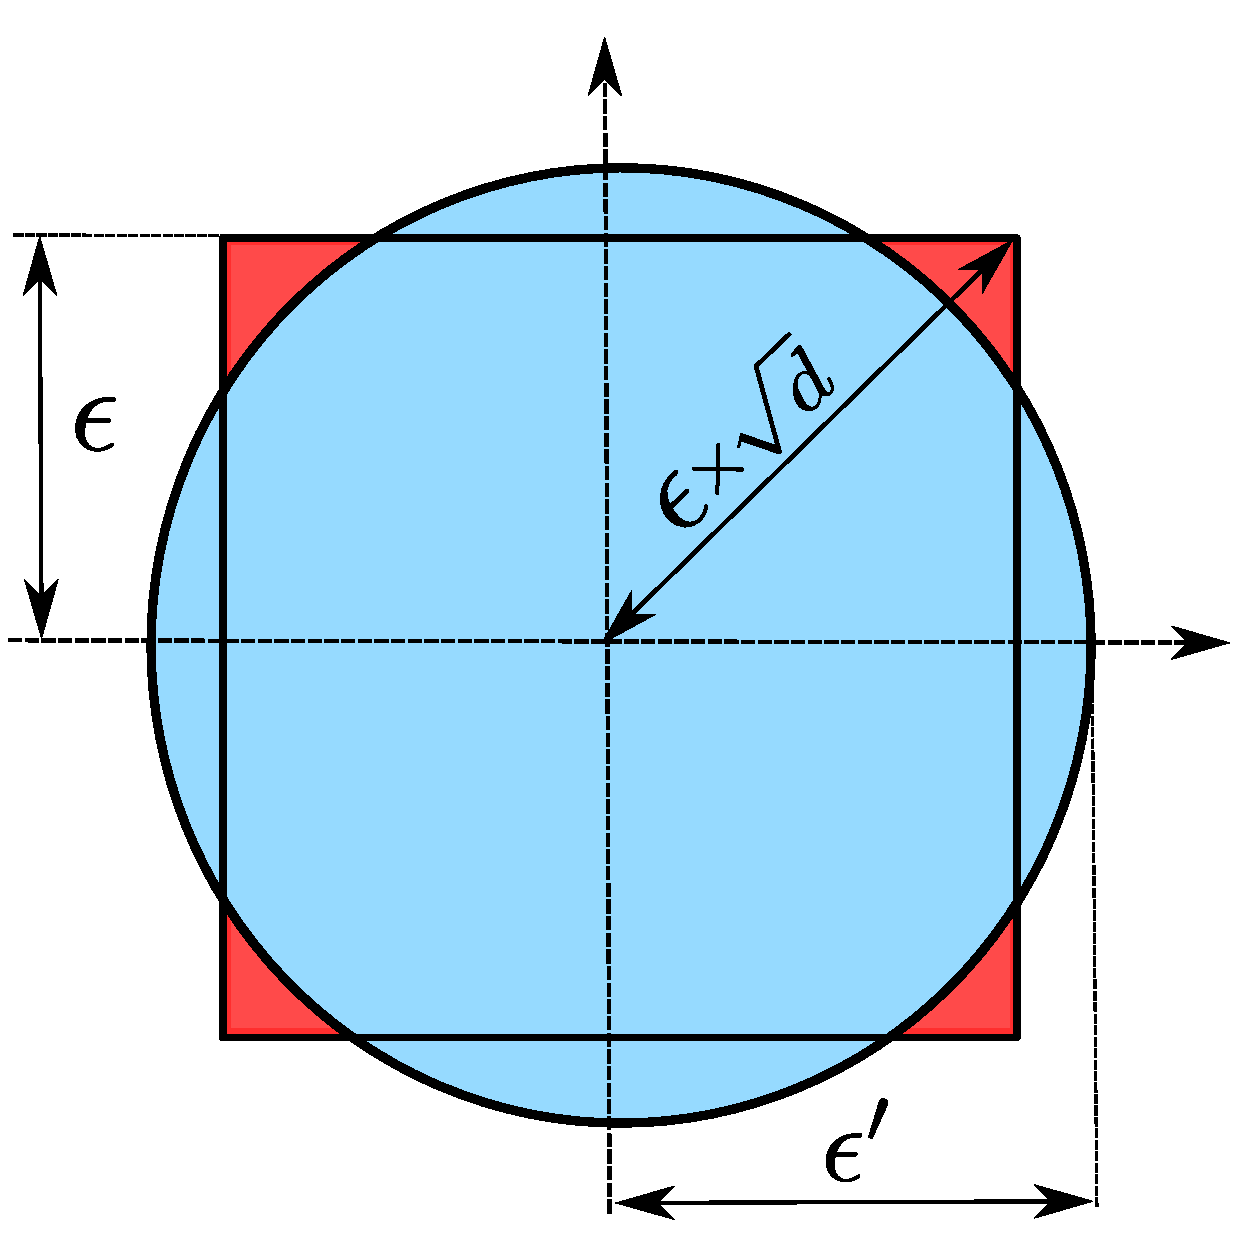
\includegraphics[scale=0.22]{figures/appendix/ap4-advocating_for_multiple_defense_strategies/ball_inclusion_adversarial_training.pdf}
       \caption{}
       \label{figure:ap4-ball_inclusion_adversarial_training}
   \end{subfigure}
   \hfill
   \begin{subfigure}[b]{0.32\textwidth}
       \centering
       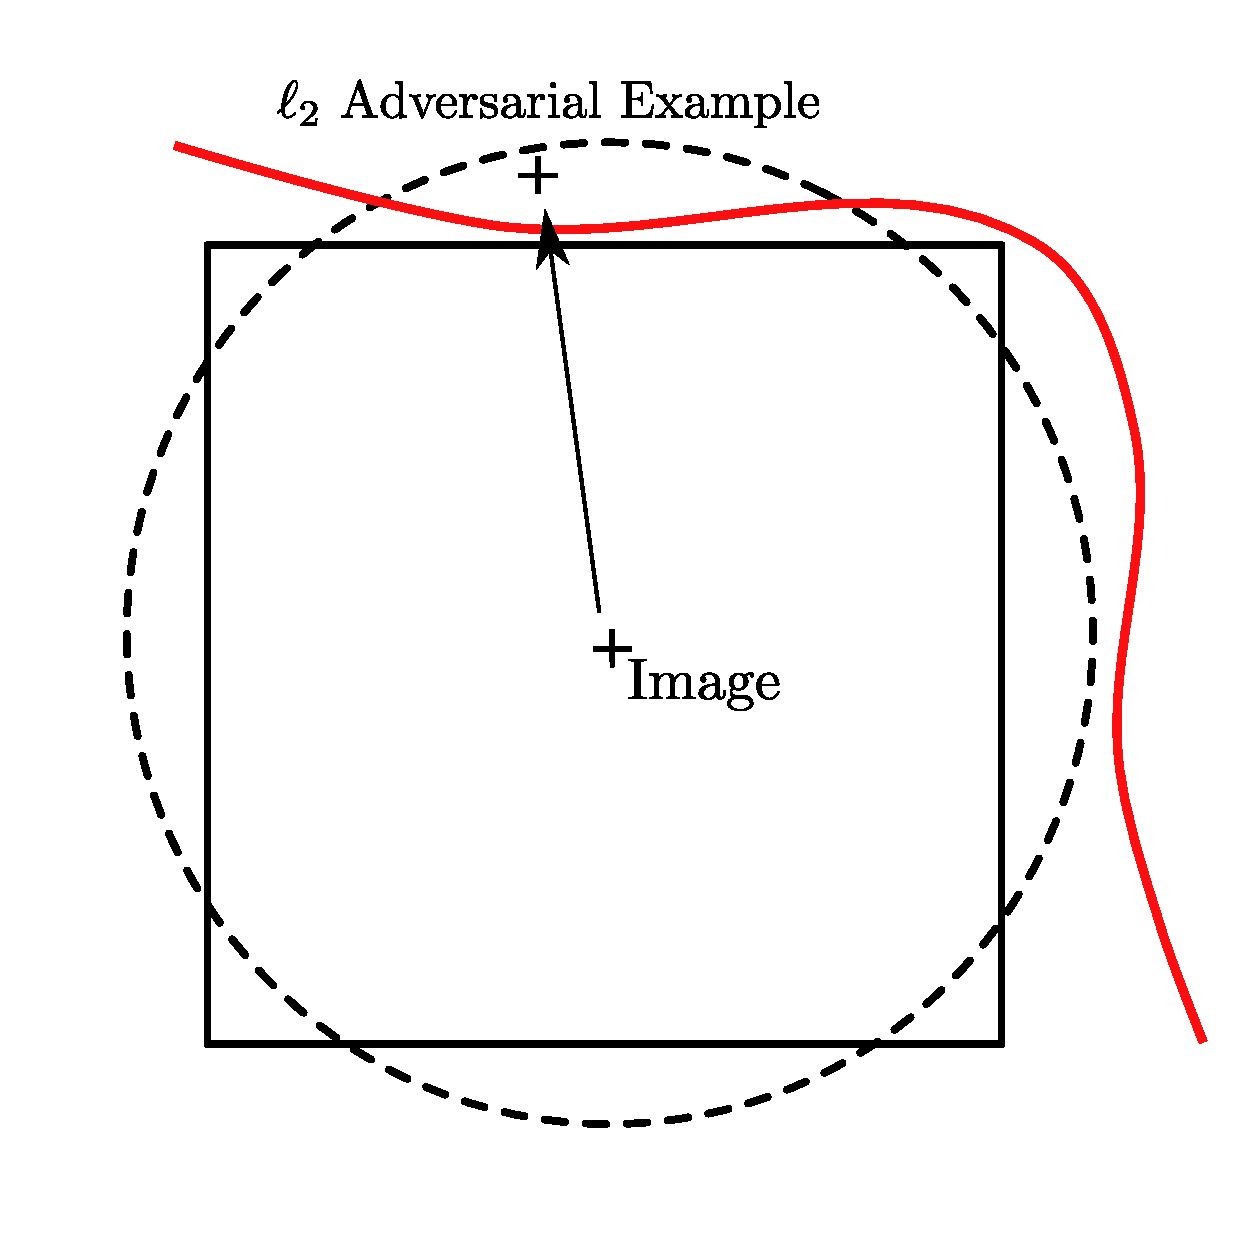
\includegraphics[scale=0.22]{figures/appendix/ap4-advocating_for_multiple_defense_strategies/ball_adversarial_l2.pdf}
       \caption{}
       \label{figure:ap4-ball_adversarial_l2}
   \end{subfigure}
   \hfill
   \begin{subfigure}[b]{0.32\textwidth}
       \centering
       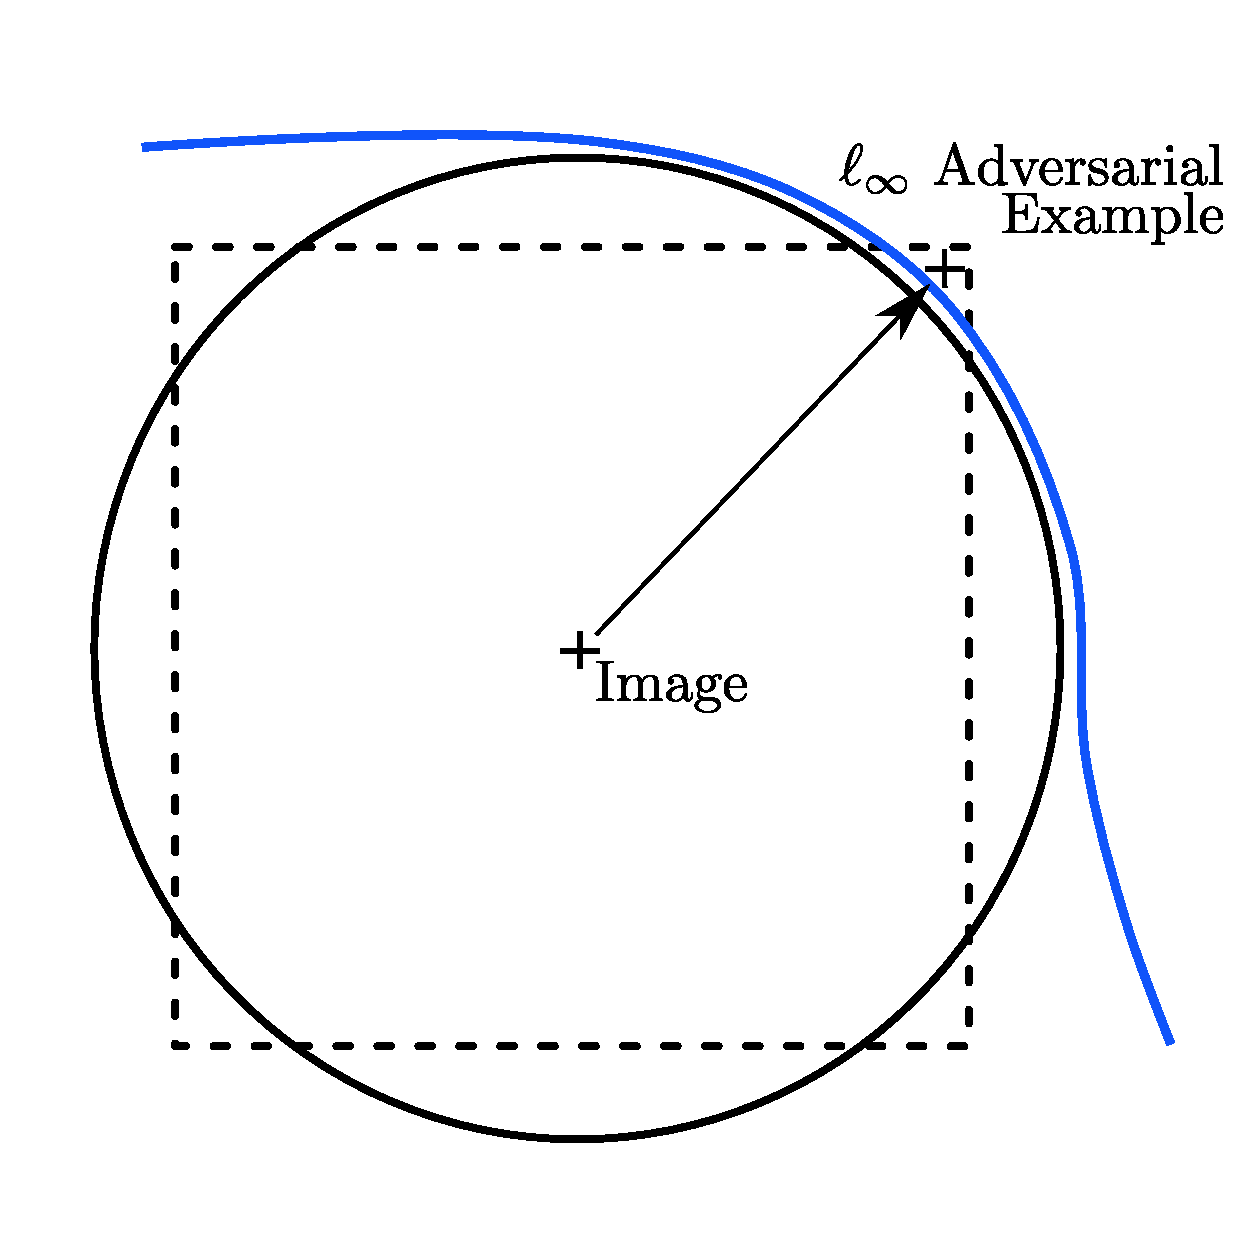
\includegraphics[scale=0.22]{figures/appendix/ap4-advocating_for_multiple_defense_strategies/ball_adversarial_linf.pdf}
       \caption{}
       \label{figure:ap4-ball_adversarial_linf}
   \end{subfigure}
   \caption{Left: 2D representation of the $\linf$ and $\ltwo$ balls of respective radius $\epsilon$ and $\epsilon'$. 
    Middle: a classifier trained with $\linf$ adversarial perturbations  (materialized by the red line) remains vulnerable to $\ltwo$ attacks. 
    Right: a classifier trained with $\ltwo$ adversarial perturbations (materialized by the blue line) remains vulnerable to $\linf$ attacks.}
\end{figure}


%%%%%%%%%%%%%%%%%%%%%%%%%%%%%%%%%%%%%%%%%%%%%%%%%%%%%%%%%%%%%%%%%%%%%%%%%%%%%%%
\subsection{Theoretical analysis}
\label{subsection:ap4-theoretical_analysis}
%%%%%%%%%%%%%%%%%%%%%%%%%%%%%%%%%%%%%%%%%%%%%%%%%%%%%%%%%%%%%%%%%%%%%%%%%%%%%%%

Let us consider a classifier $f_{\infty}$ that is provably robust against adversarial examples with maximum $\linf$ norm of value $\epsilon_\infty$.
It guarantees that for any input-output pair $(x,y) \sim \mathcal D$ and for any perturbation $\tau$ such that $\norm{\tau}_\infty \leq \epsilon_\infty$, $f_{\infty}$ is not misled by the perturbation, \ie, $f_{\infty}(x + \tau) = f_{\infty}(x)$.
We now focus our study on the performance of this classifier against adversarial examples bounded with a $\ltwo$ norm of value $\epsilon_2$.
Using Figure~\ref{figure:ap4-ball_inclusion_adversarial_training}, we observe that any $\ltwo$ adversarial example that is also in the $\linf$ ball, will not fool $f_{\infty}$.
Conversely, if it is outside the ball, we have no guarantee.

To characterize the probability that such an  $\ltwo$ perturbation fools an $\linf$ defense mechanism in the general case (\emph{i.e.}, any dimension $d$), we measure the ratio between the volume of the intersection of the $\linf$ ball of radius $\epsilon_\infty$ and the $\ltwo$ ball of radius $\epsilon_2$. As Theorem~\ref{theorem:ap4-nullvolume} shows, this ratio depends on the dimensionality $d$ of the input vector $x$, and  rapidly converges to zero when $d$ increases. 
Therefore a defense mechanism that protects against all $\linf$ bounded adversarial examples is unlikely to be efficient against $\ltwo$ attacks.


\begin{theorem}[Probability of the intersection goes to $0$] ~\\
Let
\begin{equation}
  B_{2,d}(\epsilon) \triangleq \left \{\tau \in \Rbb^d \ |\  \norm{\tau}_2 \leq \epsilon \right \}
\end{equation}
and
\begin{equation}
  B_{\infty,d}(\epsilon') \triangleq \left \{\tau \in \Rbb^d \ |\  \norm{\tau}_\infty \leq \epsilon' \right\}.
\end{equation}
If for all $d$, we select $\epsilon$ and $\epsilon$' such that $\Vol\left(B_{2,d}(\epsilon)\right) = \Vol\left(B_{\infty,d}(\epsilon')\right)$, then
\begin{equation}
  \frac{\Vol\left(B_{2,d}(\epsilon)\bigcap B_{\infty,d}(\epsilon')\right)}{\Vol\left(B_{\infty,d}(\epsilon')\right)} \rightarrow 0 \text{ when } d\rightarrow \infty.
\end{equation}
\label{theorem:ap4-nullvolume}
\end{theorem} 

\begin{proof}[\proofrefth{theorem:ap4-nullvolume}] 
Without loss of generality, let us fix $\epsilon = 1$. One can show that for all $d$, 
\begin{equation}
    \Vol\left( B_{2,d}\left(\frac{2}{\sqrt{\pi}}\Gamma\left(\frac{d}{2}+1\right)^{1/d}\right)\right) = \Vol\left(B_{\infty,d}\left(1\right)\right)
\end{equation}
where $\Gamma$ is the gamma function. Let us denote 
\begin{equation}
    r_2(d)=\frac{2}{\sqrt{\pi}}\Gamma\left(\frac{d}{2}+1\right)^{1/d}.
\end{equation}
Then, thanks to Stirling's formula
\begin{equation}
    r_2(d)\sim \sqrt{\frac{2}{\pi e}} d^{1/2}.
\end{equation}
Finally, if we denote $\mathcal{U}_S$, the uniform distribution on set $S$, by using  Hoeffding inequality between Equation~\ref{equation:ap4-hoeffding1} and \ref{equation:ap4-hoeffding2}, we get:
\begin{align}
  \frac{\Vol(B_{2,d}(r_2(d)) \bigcap B_{\infty,d}(1))}{\Vol(B_{\infty,d}(1))} &= \Pbb_{x \sim \mathcal{U}_{B_{\infty,d}(1)}} \left[ x \in B_{2,d}(r_2(d)) \right] \\
  &= \Pbb_{x \sim \mathcal{U}_{B_{\infty,d}(1)}} \left[ \sum_{i=1}^d |x_i|^2 \leq r_2^2(d) \right] \\
  &\leq \exp{- d^{-1} \left( r_2^2(d) - d \Ebb |x_1|^2 \right)^2} \label{equation:ap4-hoeffding1} \\
  &\leq \exp{-\left( \frac{2}{\pi e}-\frac23\right)^2d+o(d)} \label{equation:ap4-hoeffding2}.
\end{align}
Then the ratio between the volume of the intersection of the ball and the volume of the ball converges towards $0$ when $d$ goes to $\infty$.
\end{proof}

Theorem~\ref{theorem:ap4-nullvolume} states that, when $d$ is large enough, $\ltwo$ bounded perturbations have a null probability of being also in the $\linf$ ball of the same volume.
As a consequence, for any value of $d$ that is large enough, a defense mechanism that offers full protection against $\linf$ adversarial examples is not guaranteed to offer any protection against $\ltwo$ attacks \footnote{Theorem~\ref{theorem:ap4-nullvolume} can easily be extended to any two balls with different norms. For clarity, we restrict to the case of $\linf$ and $\ltwo$ norms.}.

\begin{table}[ht]
  \centering
  \begin{tabular}{c r r r l}
    \toprule
    \textbf{Dataset\ } & \phantom{....} & \textbf{Dim.} $\mathbf{(d)}$ & \phantom{....} & \textbf{Vol. of the intersection }\\
    \midrule
    -- & & 2\ \ & & $10^{-0.009}$ \quad ($\approx$ 0.98) \\
    MNIST & & 784\ \  & & $10^{-144}$\\
    CIFAR & & 3072\ \ & &  $10^{-578}$\\
    ImageNet & & 150528\ \ & & $10^{-28946}$\\
    \bottomrule
  \end{tabular}
  \caption{ Bounds of Theorem~\ref{theorem:ap4-nullvolume} on the volume of the intersection of  $\ltwo$ and $\linf$ balls at equal volume for typical image classification datasets. When $d=2$, the bound is $ 10^{-0.009}\approx 0.98$.}
  \label{table:ap4-datadim}
\end{table}

Note that this result defeats the 2-dimensional intuition: if we consider a 2 dimensional problem setting, the $\linf$ and the $\ltwo$ balls have an important overlap (as illustrated in Figure~\ref{figure:ap4-ball_inclusion_adversarial_training}) and the probability of sampling at the intersection of the two balls is bounded by approximately 98\%.
However, as we increase the dimensionality $d$, this probability quickly becomes negligible, even for very simple image datasets such as MNIST.
An instantiation of  the bound for classical image datasets is presented in Table~\ref{table:ap4-datadim}.
The probability of sampling at the intersection of the $\linf$ and $\ltwo$ balls is close to zero for any realistic image setting.
In large dimensions, the volume of the corner of the $\linf$ ball is much bigger than it appears in Figure~\ref{figure:ap4-ball_inclusion_adversarial_training}.


%%%%%%%%%%%%%%%%%%%%%%%%%%%%%%%%%%%%%%%%%%%%%%%%%%%%%%%%%%%%%%%%%%%%%%%%%%%%%%%
\subsection{No Free Lunch in Practice}
\label{subsection:ap4-no_free_lunch_in_practice}
%%%%%%%%%%%%%%%%%%%%%%%%%%%%%%%%%%%%%%%%%%%%%%%%%%%%%%%%%%%%%%%%%%%%%%%%%%%%%%%

Our theoretical analysis shows that if adversarial examples were uniformly distributed in a high-dimensional space, then any mechanism that perfectly defends against $\linf$ adversarial examples has a null probability of protecting against $\ltwo$-bounded adversarial attacks.
Although existing defense mechanisms do not necessarily assume such a distribution of adversarial examples, we demonstrate that whatever distribution they use, it offers no favorable bias with respect to the result of Theorem~\ref{theorem:ap4-nullvolume}.
As we discussed in Chapter~\ref{chapter:lipschitz_regularization_for_adversarial_robustness}, there are two distinct attack settings: loss maximization (PGD) and perturbation minimization (C\&W).
Our analysis is mainly focusing on loss maximization attacks.
However, these attacks have a very strict geometry\footnote{Due to the projection operator, all PGD attacks saturate the constraint, which makes them all lies in a very small part of the ball.}.
This is why, to present a deeper analysis of the behavior of adversarial attacks and defenses, we also present a set of experiments that use perturbation minimization attacks.

\begin{table}[htbp]
  \centering 
  \begin{tabular}{lrrrrrrrr}
    \toprule
      & \phantom{...}  & \multicolumn{3}{c}{Attack PGD-$\ltwo$} & \phantom{...}  & \multicolumn{3}{c}{Attack PGD-$\linf$} \\
  \cmidrule{3-5}\cmidrule{7-9}      &   & \multicolumn{1}{l}{Unprotected} &  \phantom{...} & \multicolumn{1}{l}{AT-$\linf$} &   & \multicolumn{1}{l}{Unprotected} & \phantom{...}  & \multicolumn{1}{l}{AT-$\ltwo$} \\
    \midrule
    Average $\ltwo$ norm &   & 0.830 &   & 0.830 &   & 1.400 &   & 1.640 \\
    Average $\linf$ norm &   & 0.075 &   & 0.200 &   & 0.031 &   & 0.031 \\
    \bottomrule
  \end{tabular}%
  \caption{Average norms of PGD-$\ltwo$ and PGD-$\linf$ adversarial examples with and without $\linf$ adversarial training on CIFAR-10 ($d=3072$).}
  \label{table:ap4-mean_norm_pgd_attack}
\end{table}%

\paragraph{Adversarial training vs. loss maximization attacks}

To demonstrate that $\linf$ adversarial training is not robust against PGD-$\ltwo$ attacks we measure the evolution of $\ltwo$ norm of adversarial examples generated with PGD-$\linf$ between an unprotected model and a model trained with AT-$\linf$, \ie, AT where adversarial examples are generated with PGD-$\linf$ \footnote{To do so, we use the same experimental setting as in Section~\ref{section:ap4-reviewing_defenses_against_multiple_attacks} with $\epsilon_\infty$ and $\epsilon_2$ such that the volumes of the two balls are equal.}. 
Results are presented in  Table~\ref{table:ap4-mean_norm_pgd_attack}. \footnote{All experiments in this section are conducted on CIFAR-10, and the experimental setting is fully detailed in Section~\ref{section:ap4-experimental_settings}. }

The analysis is unambiguous: the average $\linf$ norm of a bounded $\ltwo$ perturbation more than double between an unprotected model and a model trained with AT PGD-$\linf$. This phenomenon perfectly reflects the illustration of Figure~\ref{figure:ap4-ball_adversarial_linf}. The attack will generate an adversarial example on the corner of the $\linf$ ball thus increasing the $\linf$ norm while maintaining the same $\ltwo$ norm. 
We can observe the same phenomenon with AT-$\ltwo$ against PGD-$\linf$ attack (see Figure~\ref{figure:ap4-ball_adversarial_l2} and Table \ref{table:ap4-mean_norm_pgd_attack}). PGD-$\linf$ attack increases the $\ltwo$ norm while maintaining the same $\linf$ perturbation thus generating the perturbation in the upper area. 

As a consequence, we cannot expect adversarial training $\linf$ to offer any guaranteed protection against $\ltwo$ adversarial examples .

\paragraph{Adversarial training vs. perturbation minimization attacks.}
To better capture the behavior of $\ltwo$ adversarial examples, we now study the performances of an $\ltwo$ perturbation minimization attack (C\&W) with and without AT-$\linf$.
It allows us to understand in which area C\&W discovers adversarial examples and the impact of AT-$\linf$.
In high dimensions, the red corners (see Figure~\ref{figure:ap4-ball_inclusion_adversarial_training}) are very far away from the $\ltwo$ ball.
Therefore, we hypothesize that a large proportion of the $\ltwo$ adversarial examples will remain unprotected.
To validate this assumption, we measure the proportion of adversarial examples inside of the $\ltwo$ ball before and after $\linf$ adversarial training.
The results are presented in Figure~\ref{fig:calotte} (left: without adversarial training, right: with adversarial training). 

\begin{figure}[htb]
    \centering
    \begin{tikzpicture}[scale=0.7]
    \begin{groupplot}[group style={
                        group name=myplot,
			group size= 2 by 1,
		        horizontal sep=3cm},
                      grid style=dashed,
		      ymajorgrids=true]
       
    \nextgroupplot[
       stack plots=y,
       area style,
       ytick={0,5000,1000},
       ymin=0,
       ymax=10000,
       xmin=0.3,
       xmax=16.63,
       axis x line*=bottom,
       axis y line*=left,
       xtick={2,14},
       xticklabels={\Large $\epsilon'=\epsilon\phantom{\sqrt{d}}$, \Large $\epsilon'=\epsilon\times\sqrt{d}$},
       xtick style={draw=none}]
        \addplot table [x=eps,y=linf_ball] {figures/appendix/ap4-advocating_for_multiple_defense_strategies/data/ball_l2_base.dat}\closedcycle;
        \addplot table [x=eps,y=callote] {figures/appendix/ap4-advocating_for_multiple_defense_strategies/data/ball_l2_base.dat}\closedcycle;
        \addplot table [x=eps,y=outside] {figures/appendix/ap4-advocating_for_multiple_defense_strategies/data/ball_l2_base.dat}\closedcycle;

    \nextgroupplot[
       stack plots=y,
       area style,
       ytick={0,5000,1000},
       ymin=0,
       ymax=10000,
       xmin=0.3, 
       xmax=16.63,
       axis x line*=bottom,
       axis y line*=left,
       xtick={2,14},
       xticklabels={\Large $\epsilon'=\epsilon\phantom{\sqrt{d}}$, \Large $\epsilon'=\epsilon\times\sqrt{d}$},
       xtick style={draw=none}]
        \addplot table [x=eps,y=linf_ball] {figures/appendix/ap4-advocating_for_multiple_defense_strategies/data/ball_l2_at.dat}\closedcycle;
        \addplot table [x=eps,y=callote] {figures/appendix/ap4-advocating_for_multiple_defense_strategies/data/ball_l2_at.dat}\closedcycle;
        \addplot table [x=eps,y=outside] {figures/appendix/ap4-advocating_for_multiple_defense_strategies/data/ball_l2_at.dat}\closedcycle;

    \end{groupplot}
\end{tikzpicture}


    \caption{Comparison of the number of adversarial examples found by C\&W, inside the $\linf$ ball (lower, blue area), outside the $\linf$ ball but inside the $\ltwo$ ball (middle, red area) and outside the $\ltwo$ ball (upper gray area). $\epsilon$ is set to $0.3$ and $\epsilon'$ varies along the x-axis. Left: without adversarial training, right: with adversarial training. Most adversarial examples have shifted from the $\linf$ ball to the cap of the $\ltwo$ ball, but remain at the same $\ltwo$ distance from the original example.}
    \label{fig:calotte}
\end{figure}

On both charts, the blue area represents the proportion of adversarial examples that are inside the $\linf$ ball.
The red area represents the adversarial examples that are outside the $\linf$ ball but still inside the $\ltwo$ ball (valid $\ltwo$ adversarial examples).
Finally, the brown-beige area represents the adversarial examples that are beyond the $\ltwo$ bound.
The radius $\epsilon'$ of the $\ltwo$ ball varies along the x-axis from $\epsilon'$ to $\epsilon' \sqrt{d}$.
On the left chart (without adversarial training) most $\ltwo$ adversarial examples generated by C\&W are inside both balls.
On the right chart most of the adversarial examples have been shifted out the $\linf$ ball.
This is the expected consequence of $\linf$ adversarial training.
However, these adversarial examples remain in the $\ltwo$ ball, \ie, they are in the cap of the $\ltwo$ ball.
These examples are equally good from the $\ltwo$ perspective.
This means that even after adversarial training, it is still easy to find good $\ltwo$ adversarial examples, making the $\ltwo$ robustness of AT-$\linf$ almost null. 

%%%%%%%%%%%%%%%%%%%%%%%%%%%%%%%%%%%%%%%%%%%%%%%%%%%%%%%%%%%%%%%%%%%%%%%%%%%%%%%%
\section{Reviewing Defenses Against Multiple Attacks}
\label{section:ap4-reviewing_defenses_against_multiple_attacks}
%%%%%%%%%%%%%%%%%%%%%%%%%%%%%%%%%%%%%%%%%%%%%%%%%%%%%%%%%%%%%%%%%%%%%%%%%%%%%%%%

\begin{table}[htbp]
  \centering
  \begin{tabular}{lccccccccccccccccc}
    \toprule
      &   & \textbf{Baseline} & \phantom{...}  & \multicolumn{2}{c}{\textbf{AT}} & \phantom{...}  & \multicolumn{2}{c}{\textbf{MAT}} &  \phantom{...} & \multicolumn{2}{c}{\textbf{NI}} &  \phantom{...} & \multicolumn{2}{c}{\textbf{RAT}-$\linf$} &  \phantom{...} & \multicolumn{2}{c}{\textbf{RAT}-$\ltwo$} \\
  \cmidrule{3-3}\cmidrule{5-6}\cmidrule{8-9}\cmidrule{11-12}\cmidrule{14-15}\cmidrule{17-18}      &   & -- &   & $\linf$ & $\ltwo$ &   & Max & Rand &   & $\mathcal{N}$ & $\mathcal{U}$ &   & $\mathcal{N}$ & $\mathcal{U}$ &   & $\mathcal{N}$ & $\mathcal{U}$ \\
    \midrule
    Natural &   & 0.94 &   & 0.85 & 0.85 &   & 0.80 & 0.80 &   & 0.79 & 0.87 &   & 0.74 & 0.80 &   & 0.79 & 0.87 \\
    PGD-$\linf$ &   & 0.00 &   & 0.43 & 0.37 &   & 0.37 & 0.40 &   & 0.23 & 0.22 &   & 0.35 & 0.40 &   & 0.23 & 0.22 \\
    PGD-$\ltwo$ &   & 0.00 &   & 0.37 & 0.52 &   & 0.50 & 0.55 &   & 0.34 & 0.36 &   & 0.43 & 0.39 &   & 0.34 & 0.37 \\
    \bottomrule
  \end{tabular}%
  \caption{This table shows a comprehensive list of results consisting of the accuracy of several defense mechanisms against $\ltwo$ and $\linf$ attacks. This table main objective is to compare the overall performance of ‘single‘ norm defense mechanisms (AT and NI presented in the Chapter~\ref{chapter:75748} Section~\ref{section:96537834}) against mixed norms defense mechanisms (MAT \& RAT mixed defenses presented in Section~\ref{section:ap4-reviewing_defenses_against_multiple_attacks}).}
  \label{table:ap4-results}
\end{table}%

Adversarial attacks have been an active topic in the machine learning community since their discovery~\cite{globerson2006nightmare, biggio2013evasion,szegedy2013intriguing}.
Many attacks have been developed.
Most of them solve a loss maximization problem with either $\linf$~\cite{goodfellow2014explaining,kurakin2016adversarial,madry2018towards}, $\ltwo$~\cite{carlini2017towards,kurakin2016adversarial,madry2018towards}, $\lone$~\cite{tramer2019adversarial} or $\lzero$~\cite{papernot2016limitations} surrogate norms.
As we showed, these norms are really different in high dimension.
Hence, defending against one norm-based attack is not sufficient to protect against another one. 
In order to solve this problem, we review several strategies to build defenses against multiple adversarial attacks.
These strategies are based on the idea that both types of defense must be used simultaneously in order for the classifier to be protected against multiple attacks.
The detailed description of the experimental setting is described in Section~\ref{section:ap4-experimental_settings}.

%%%%%%%%%%%%%%%%%%%%%%%%%%%%%%%%%%%%%%%%%%%%%%%%%%%%%%%%%%%%%%%%%%%%%%%%%%%%%%%
\subsection{Experimental Setting}
\label{section:ap4-experimental_settings}
%%%%%%%%%%%%%%%%%%%%%%%%%%%%%%%%%%%%%%%%%%%%%%%%%%%%%%%%%%%%%%%%%%%%%%%%%%%%%%%

To compare the robustness provided by the different defense mechanisms, we use strong adversarial attacks and a conservative setting: the attacker has a total knowledge of the parameters of the model (white-box setting) and we only consider untargeted attacks  (a misclassification from one target to any other will be considered as adversarial).
To evaluate defenses based on Noise Injection, we use {\em Expectation Over Transformation} (EOT), the rigorous experimental protocol  proposed by \cite{athalye2017synthesizing} and later used by \cite{athalye2018obfuscated,carlini2019evaluating} to identify flawed defense mechanisms. 

To attack the models, we use state-of-the-art algorithms PGD.
We run PGD with 20 iterations to generate adversarial examples and with 10 iterations when it is used for adversarial training.
The maximum $\linf$ bound is fixed to $0.031$ and the maximum $\ltwo$ bound is fixed to $0.83$.
We chose these values so that the $\linf$ and the $\ltwo$ balls have similar volumes.
Note that $0.83$ is slightly above the values typically used in previous publications in the area, meaning the attacks are stronger, and thus  more difficult to defend against.

All experiments are conducted on CIFAR-10 with the Wide-Resnet 28-10 architecture.
We use the training procedure and the hyper-parameters described in the original paper by~\cite{zagoruyko2016wide}.
Training time varies from 1 day (AT) to 2 days (MAT) on 4 GPUs-V100 servers. 


%%%%%%%%%%%%%%%%%%%%%%%%%%%%%%%%%%%%%%%%%%%%%%%%%%%%%%%%%%%%%%%%%%%%%%%%%%%%%%%
\subsection{MAT -- Mixed Adversarial Training}
\label{subsection:ap4-mixed_adversarial_training}
%%%%%%%%%%%%%%%%%%%%%%%%%%%%%%%%%%%%%%%%%%%%%%%%%%%%%%%%%%%%%%%%%%%%%%%%%%%%%%%

Earlier results have shown that AT-$\lp$ improves the robustness against corresponding $\lp$-bounded adversarial examples, and the experiments we present in this section corroborate this observation (See Table~\ref{table:ap4-results}, column: AT).
Building on this, it is natural to examine the efficiency of \emph{Mixed Adversarial Training} (MAT) against mixed $\linf$ and $\ltwo$ attacks.
MAT is a variation of AT that uses both $\linf$-bounded adversarial examples and $\ltwo$-bounded adversarial examples as training examples.
As discussed in~\cite{tramer2019adversarial}, there are several possible strategies to mix the adversarial training examples.
The first strategy (MAT-Rand) consists in randomly selecting one adversarial example among the two most damaging $\linf$ and $\ltwo$, and to use it as a training example, as described in Equation~(\ref{eq:mat-rand}): 

\paragraph{MAT-Rand}:
\begin{equation}
  \min_{\theta} \Ebb_{(x, y) \sim \mathcal{D}} \left[\Ebb_{p\sim\mathcal{U}({\{2, \infty\})}} \max_{\norm{\tau}_p \leq \epsilon} \mathcal{L} \left( f_{\theta}(x+\tau), y \right) \right].
  \label{eq:mat-rand}
\end{equation}

An alternative strategy is to systematically train the model with the most damaging adversarial example ($\linf$ or $\ltwo$). As described in Equation~(\ref{eq:mat-max}): 

\paragraph{MAT-Max}:
\begin{equation}
    \min_{\theta} \Ebb_{(x, y) \sim \mathcal{D}} \left[ \max_{p \in \{2, \infty\}} \max_{\norm{\tau}_p \leq \epsilon} \mathcal{L} \left( f_{\theta}(x+\tau), y \right) \right].
    \label{eq:mat-max}
\end{equation}

The accuracy of MAT-Rand and MAT-Max are reported in Table~\ref{table:ap4-results} (Column: MAT).
As expected, we observe that MAT-Rand and MAT-Max offer better robustness both against PGD-$\ltwo$ and PGD-$\linf$ adversarial examples than the original AT does.
More  generally, we can see that AT is a good strategy against loss maximization attacks, and thus it is not surprising that MAT is a good strategy against mixed loss maximization attacks.
However efficient in practice, MAT (for the same reasons as AT) lacks theoretical arguments.
In order to get the best of both worlds, \cite{salman2019provably} proposed to mix adversarial training with randomization.  


%%%%%%%%%%%%%%%%%%%%%%%%%%%%%%%%%%%%%%%%%%%%%%%%%%%%%%%%%%%%%%%%%%%%%%%%%%%%%%%
\subsection{RAT -- Randomized Adversarial Training}
\label{subsection:ap4-randomized_adversarial_training}
%%%%%%%%%%%%%%%%%%%%%%%%%%%%%%%%%%%%%%%%%%%%%%%%%%%%%%%%%%%%%%%%%%%%%%%%%%%%%%%

We now examine the performance of Randomized Adversarial Training (RAT) first introduced in~\cite{salman2019provably}.
This technique mixes Adversarial Training with Noise Injection.
The corresponding loss function is defined as follows:
\begin{equation}
  \min_{\theta} \Ebb_{(\xvec, y) \sim \mathcal{D}} \left[ \max_{\norm{\tau}_p \leq \epsilon} \mathcal{L} \left( \tilde{f}_{\theta}(\xvec+\tau), y)  \right) \right].
\end{equation}
where $\tilde{f}_\theta$ is a randomized neural network with noise injection as described in Section~\ref{subsection:ch6-randomized_training}, and $\norm{\ \cdot\ }_p$ define which kind of AT is used.
For each setting, we consider two noise distributions, Gaussian and Uniform as we did with NI.
We also consider two different Adversarial training AT-$\linf$ as well as AT-$\ltwo$. 

The results of RAT are reported in Table~\ref{table:ap4-results}~(Columns: RAT-$\linf$ and RAT-$\ltwo$).
We can observe that RAT-$\linf$ offers the best extra robustness with both noises, which is consistent with previous experiments, since AT is generally more effective against $\linf$ attacks whereas NI is more effective against $\ltwo$-attacks.
Overall, RAT-$\linf$ and a noise from uniform distribution offers the best performances but is still weaker than MAT-Rand.
These results are also consistent with the literature, since adversarial training (and its variants) is the best defense against adversarial examples so far.


%%%%%%%%%%%%%%%%%%%%%%%%%%%%%%%%%%%%%%%%%%%%%%%%%%%%%%%%%%%%%%%%%%%%%%%%%%%%%%%
\section{Conclusion}
\label{section:ap4-conclusion}
%%%%%%%%%%%%%%%%%%%%%%%%%%%%%%%%%%%%%%%%%%%%%%%%%%%%%%%%%%%%%%%%%%%%%%%%%%%%%%%

In this paper, we tackled the problem of protecting neural networks against multiple attacks crafted from different norms.
We demonstrated and gave a geometrical interpretation to explain why most defense mechanisms can only protect against one type of attack.
Then we reviewed existing strategies that mix defense mechanisms in order to build models that are robust against multiple adversarial attacks.
We conduct a rigorous and full comparison of \emph{Randomized Adversarial Training} and \emph{Mixed Adversarial Training} as defenses against multiple attacks.

We could argue that both techniques offer benefits and limitations.
We have observed that MAT offers the best empirical robustness against multiples adversarial attacks but this technique is computationally expensive which hinders its use in large-scale applications.
Randomized techniques have the important advantage of providing theoretical guarantees of robustness and being computationally cheaper.
However, the certificate provided by such defenses is still too small for strong attacks.
Furthermore, certain Randomized defenses also suffer from the curse of dimensionality as recently shown by \cite{kumar2020curse}. 

Although, randomized defenses based on noise injection seem limited in terms of accuracy under attack and scalability, they could be improved either by Learning the best distribution to use or by leveraging different types of randomization such as discrete randomization first proposed in \cite{pinot2020randomization}.
We believe that these certified defenses are the best solution to ensure the robustness of classifiers deployed into real-world applications.

